%Por favor no editar esta plantilla, sino guardarla con otro nombre y luego si realizar los cambios que se desee
\documentclass[conference]{IEEEtran}
% Esto es para que el LaTeX sepa que el texto está en español:
\usepackage[spanish,mexico]{babel}
\selectlanguage{spanish}
% Esto es para poder escribir acentos directamente:
\usepackage[utf8]{inputenc}
\usepackage[T1]{fontenc}
\usepackage{hyperref}
\usepackage{breakurl}
\usepackage{amsmath}
\label{usepackage}
\usepackage[latin1]{inputenc} %Acentos
\usepackage{algorithmic} %Algoritmos
\usepackage{graphicx} %Gráficas

\begin{document}
%Para modificar el titulo se debe abrir y editar el archivo Titulo.tex
\title{\\Calibracion y Adquisición de Datos} \label{sec:titulo}

\author{
\IEEEauthorblockN{1\textsuperscript{st} Juan Cepeda}
\IEEEauthorblockA{\textit{Ingeniería Mecatrónica} \\
\textit{Universidad ECCI}\\
Bogotá, Colombia\\
juanp.cepedag@ecci.ecu.co}
\and
\IEEEauthorblockN{2\textsuperscript{st} Javier Gamboa}
\IEEEauthorblockA{\textit{Ingeniería Mecatrónica} \\
\textit{Universidad ECCI}\\
Bogotá, Colombia\\
javiers.gamboab@ecci.ecu.co}
\and
\IEEEauthorblockN{3\textsuperscript{st} Wilson Garcia}
\IEEEauthorblockA{\textit{Ingeniería Mecatrónica} \\
\textit{Universidad ECCI}\\
Bogotá, Colombia\\
wilsona.garcial@ecci.ecu.co}
}

\maketitle
\begin{abstract}
 En el presente trabajo, se usa un sensor inercial
MPU6050 junto con una tarjeta STM32F411 para obtener y calibrar los datos del sensor de ella como
son giroscopio y acelerómetro cuando están en estado
horizontalmente estático. En la primera parte encontramos
definiciones relevantes para la comprensión del documento,
en la siguiente parte del trabajo, características de la
código con el que se realizará la adquisición y calibración
de los datos, de la misma manera los valores de
desplazamiento para cada eje de los sensores descritos anteriormente,
ya que con esto procedemos a continuar el laboratorio
Para llevar a cabo el objetivo del laboratorio, se ha utilizado
un monitor serial  y una interfaz Matlab para ver
y analizar los datos del sensor en la pantalla y realizar la
calibración correspondiente. Debajo están los
resultados adquiridos en el procesamiento de datos en ellos
el análisis de datos no calibrados y calibrados se realiza en dos
formas en un marco de datos y otro de forma gráfica.
Finalmente, se encontraron las conclusiones sobre los hallazgos
encontrados en los datos y dificultades que tienen
en la realización de todo el laboratorio.     
\end{abstract}
 


\\
%Se colocan a continuación las palabras claves
\begin{IEEEkeywords}
    Adquisición, calibración, comunicación,  
\end{IEEEkeywords}
%De aquí en adelante van las diferentes secciones del artículo
%Para modificar el resumen se debe abrir y editar el archivo Resumen.tex
\section{Introducción} \label{sec:introduccion}


El siguiente documento contiene los temas dirigidos a
adquisición y procesamiento de datos en el MPU6050
que se trabajó a través de su hoja de datos, en la que
explica todo el funcionamiento de esto y cómo es el camino
apropiado para usar los sensores, esto se hará de acuerdo
a los códigos y ejemplos generados por el profesor y
idealmente aplicado por el estudiante haciendo un
análisis y comprensión de ellos para su implementación en
trabajos futuros También se realiza un análisis de las obras.
llevado a cabo en el procesamiento de datos con el
MPU6050 en el que se intervienen los sensores del acelerómetro
y giroscopio para tener una mayor apropiación del tema y
para poder llevar el trabajo a un mejor desarrollo.

%Para modificar la introducción se debe abrir y editar el archivo Introduccion.tex

%Para modificar los resultados se debe abrir y editar el archivo MarcoTeorico.tex
\section{Marco Teórico} \label{sec:marcoteorico}
MPU6050: es una unidad de medida inercial o IMU de 6
grados de libertad, ya que combina un acelerómetro de 3 ejes
y un giroscopio de 3 ejes. Este sensor es ampliamente utilizado en
navegación, goniometría, estabilización, etc.

Acelerómetro: es un dispositivo que mide la vibración o
La aceleración del movimiento de una estructura.

Giroscopio: es un dispositivo mecánico utilizado para medir,
mantener o cambiar la orientación en el espacio de algunos
electrodoméstico o vehículo. 
\begin{figure}[htbp]
\centering
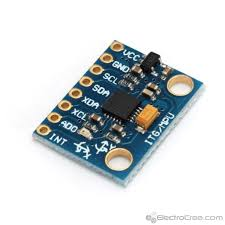
\includegraphics[width=5cm]{Figuras/acelerometro}
\caption{MPU6050 (Acelerometro y Giroscopio)}
\label{fig:acelerometro}
\end{figure}

Raspberry PI: es una placa computadora (SBC) de bajo coste, se podría decir que es un ordenador de tamaño reducido, del orden de una tarjeta de crédito, desarrollado en el Reino Unido por la Fundación Raspberry PI (Universidad de Cambridge) en 2011, con el objetivo de estimular la enseñanza de la informática en las escuelas, aunque no empezó su comercialización hasta el año 2012. \cite{vujovic2015raspberry}

\begin{figure}[htbp]
\centering
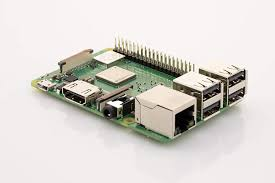
\includegraphics[width=5cm]{Figuras/rapsberry}
\caption{Rapsberry PI}
\label{fig:rapsberry}
\end{figure}

Puerto serie: es un módulo de comunicación digital para
un sistema integrado, es decir, permite la comunicación entre
Dos dispositivos digitales. Tiene dos conexiones, RX y
TX. Lo que indica los modos de comunicación que pueden
manejar, Full-duplex, Duplex y Simplex.

Sensibilidad: se refiere a la respuesta que el instrumento
la medición tiene que medir una variable y qué tan rápido es
esto para estabilizar su medida. 

VNC: Computación de red virtual. Es un programa de software gratuito basado en una estructura cliente-servidor que permite
observar las acciones de la computadora del servidor de forma remota para a través de una computadora cliente \cite{velasquez2013monitoreo}.

I2C: es un puerto y protocolo de comunicación serial, define
trama de datos y conexiones físicas para transferir bits
entre 2 dispositivos digitales. El puerto incluye dos cables.
comunicación, SDA y SCL. Además el protocolo permite
conecta hasta 127 dispositivos esclavos a esas dos líneas,
con velocidades de hasta 100, 400 y 1000 kbits / s.
\begin{figure}[htbp]
\centering
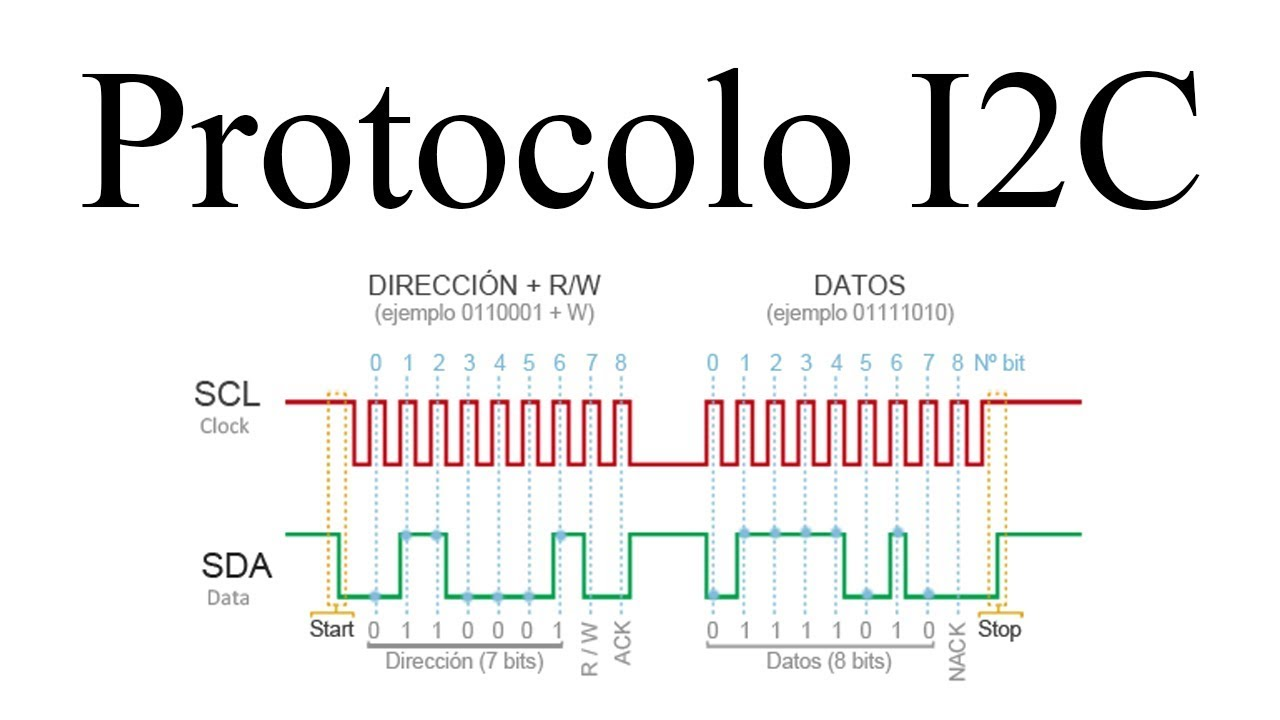
\includegraphics[width=7cm]{Figuras/I2C}
\caption{Protocolo I2C}
\label{fig:I2C}
\end{figure}




%Para modificar los resultados se debe abrir y editar el archivo Metodologia.tex
\section{Metodología} \label{sec:metodologia}

Se realiza un código en embed que ayudara en primer lugar a la adquisición de datos de la IMU (MPU6050) por medio de la tarjeta STM32F446 mediante los pines RX y TX (PA2 y PA3) que servirá para obtener las lecturas de 3 sensores como lo son acelerómetro giroscopio y temperatura que se podrán ver utilizando el puerto COM con cualquier visualizador de datos en este caso el que trae por defecto el software de arduino, así como su segunda funcionalidad que es activar la comunicación serial (UART) para lograr una conexión en este caso el PC por el mismo puerto ya mencionado, para posteriormente utilizar el software matlab que nos servirá de procesamiento de datos y genracion de gráficos \cite{elizondo2002matlab} como el ejercicio lo exige, para por ultimo realizar el análisis de las gráficas luego de un proceso de calibrado \cite{wolf1992precision} de las mediciones realizadas por el giroscopio en grado, el acelerómetro en unidades de m/s2 en las ejes X,Y y Z y como un adición la temperatura pero para este ultimo no se realizara análisis con un comportamiento gráfico únicamente ser revisara si se realiza la calibración.

%Para modificar los resultados se debe abrir y editar el archivo Resultados.tex
\section{Resultados} \label{sec:resultados}
En primer lograr obtendremos lo valores en el visualizador de arduino de la tarjeta IMU sin calibrar \cite{segovia2018adquisicion} que como se observo presentan desvios ya que en el caso del acelerometro los del eje X resultados cercanos a 0.5 y en Y -0.02, en el caso de su eje Z si se encuentran muy cercanos a 1 pero presentan una pequeña impresicion como lo es 0.98, para giroscopio se necesitara que los valores se encuentren cercanos a = pero para los tres ejes obtenes valores como -4.72, 1.38 y -0.13 en el eje z.\\
En comparación a los datos que se obtuvieron luego de modificar los offset \cite{rodriguez2001introduccion} y calibrar los valores que como se observar en la siguiente imagen obtenemos mejores comportamientos como lo son para el Acelerometro en sus ejes X y Y valores un poco mas cercanos a cero como lo son 0.01 y -0.01, para el eje Z valores entre 0.99 y 1.00. Por ultimo se observa el comportamiento de los valores en el giroscopio en sus 3 ejes X,Y y Z de 0.01,0.18 y 0.29 estos datos fueron depositados en una sola imagen ya que modificando el codigo se logra la visualización de los datos sin calibrar y calibrados por ello se observan 12 datos en la Fig.4

\begin{figure}[htbp]
\centering
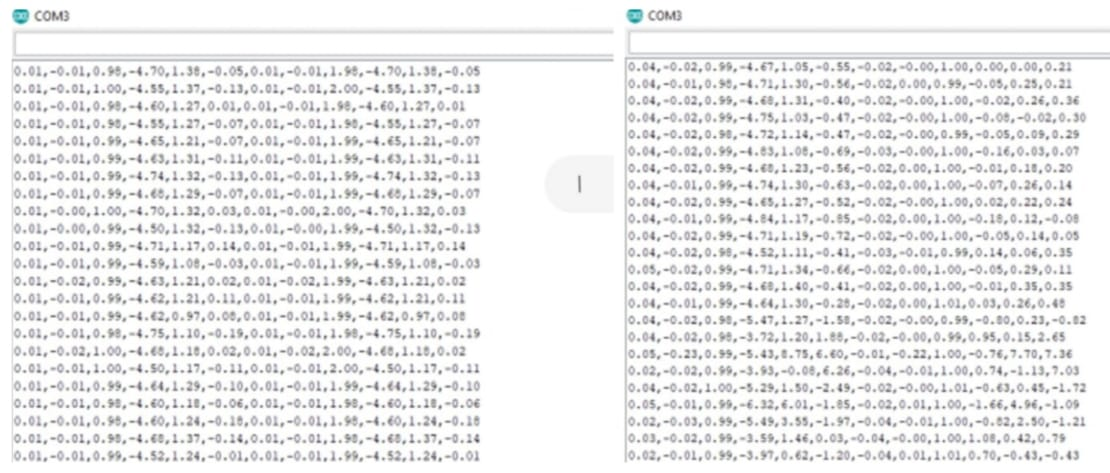
\includegraphics[width=8cm]{Figuras/calibrados_sincalibrar.jpg}
\caption{Datos sin calibrar/ Datos calibrados}
\label{fig:calibrados_sincalibrar}
\end{figure}

A continuación se podrá realizar el análisis visual de la gráfica (Fig.5) y el comportamiento de los datos sin calibrar del acelerómetro donde se observa claramente lo mencionado anteriormente que los valores de los ejes X y Y se encuentran un poco desviados de su punto de precisión 0 y igual para la linea delineada de verde que nos simboliza el eje z vemos como principio se encuentra muy cercana a 1 y finalizando ya se encuentra mas alejada del setpoint mencionado.
\begin{figure}[htbp]
\centering
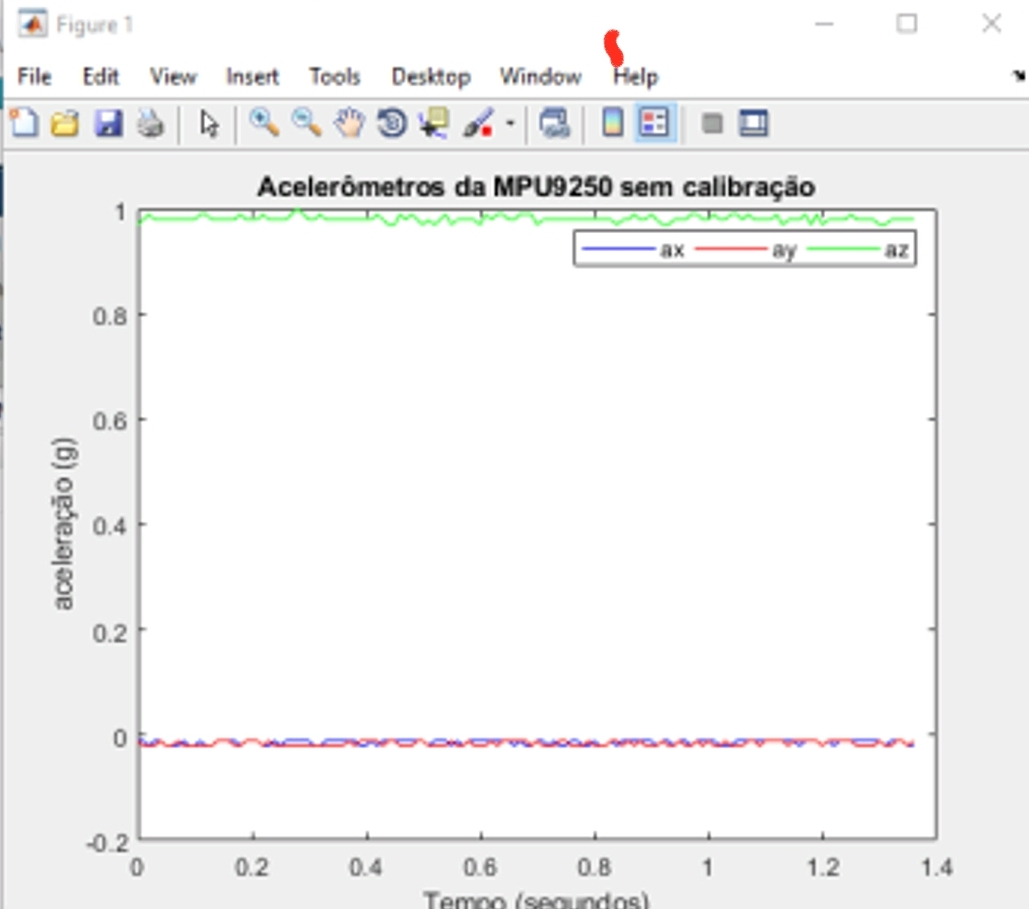
\includegraphics[width=7cm]{Figuras/acelerometro sin calibrar.jpeg}
\caption{Grafica de acelerometro sin calibrar}
\label{fig:acelerometro sin calibrar}
\end{figure}\\
Luego del proceso de ajuste o calibracionde las variables se ve claramente un mejor comportamiento de las variables X y Y practimente en 0 y la variable Z completamente en valores de 1 en la Fig.6.
\begin{figure}[htbp]
\centering
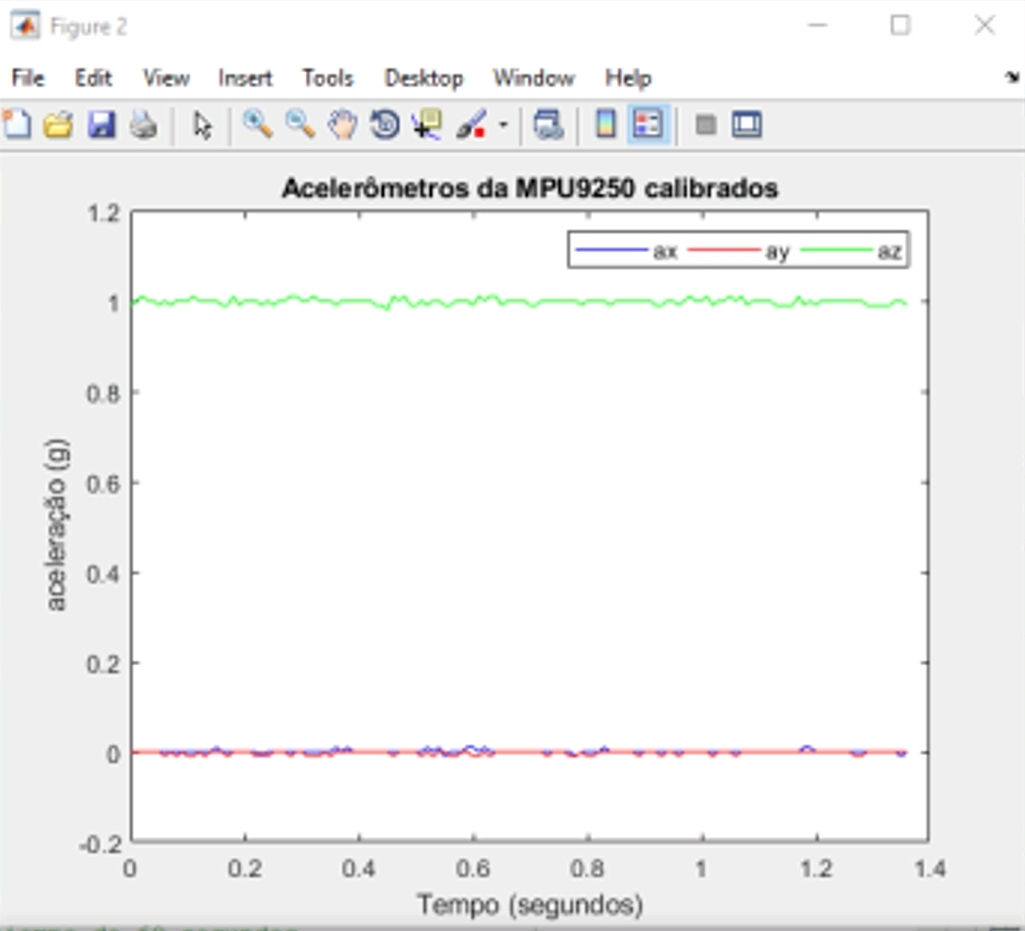
\includegraphics[width=7cm]{Figuras/acelerometro calibrado.jpeg}
\caption{Gráfica de acelerómetro calibrado}
\label{fig:acelerometro calibrado}
\end{figure}\\
En la Fig.7 se observa que la velocidad angular a las que responde el sensor se encuentran completamente desviadas en todos sus ejes pero el que mas requeria de calibracion era la variable del eje x que se encontraba cerca a los -5 m/s representado por una linea azul.\\
\begin{figure}[htbp]
\centering
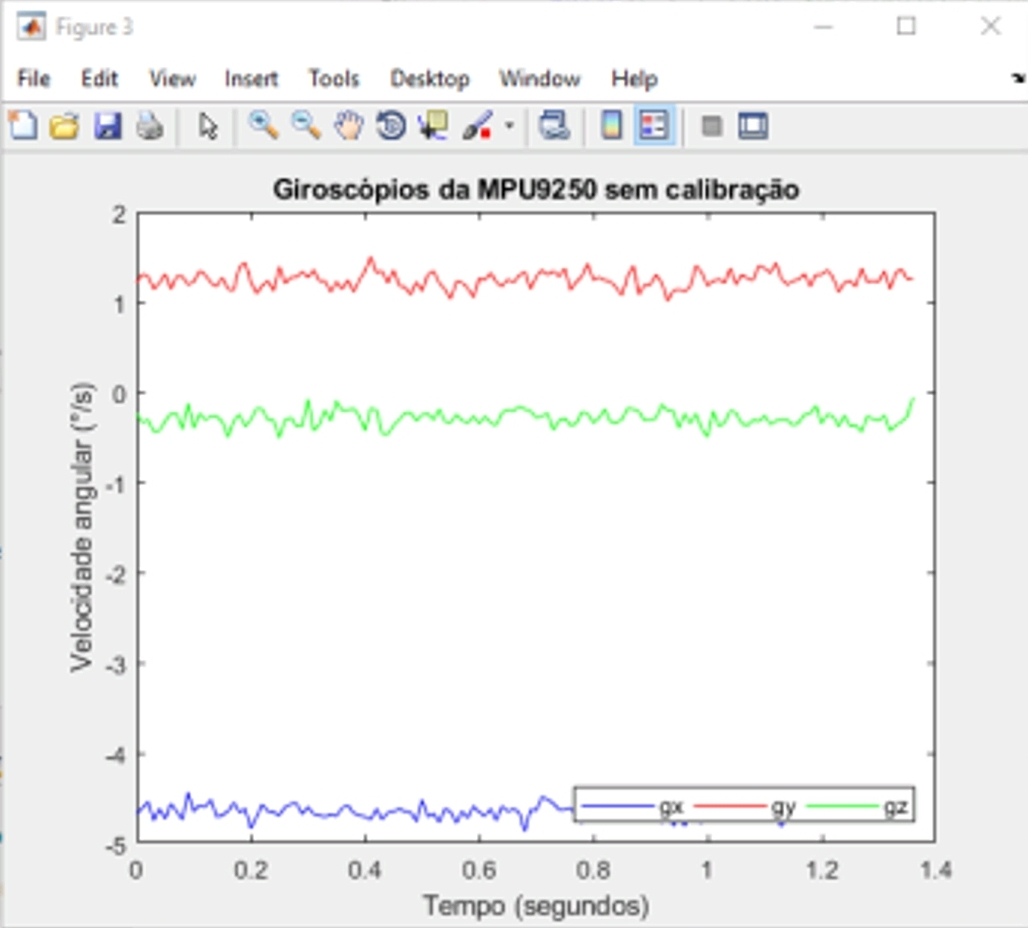
\includegraphics[width=7cm]{Figuras/giroscopio sin calibrar.jpeg}
\caption{Gráfica del giroscopio sin calibrar}
\label{fig:giroscopio sin calibrar}
\end{figure}
Luego de realizar la calibración pertinente igualmente como sucedió con el acelerómetro obtenemos en la gráfica de la Fig.8 una respuesta totalmente precisa ya que los valores se encuentran muy cercanos a 0 como se veía en los datos del visualizador
\begin{figure}[htbp]
\centering
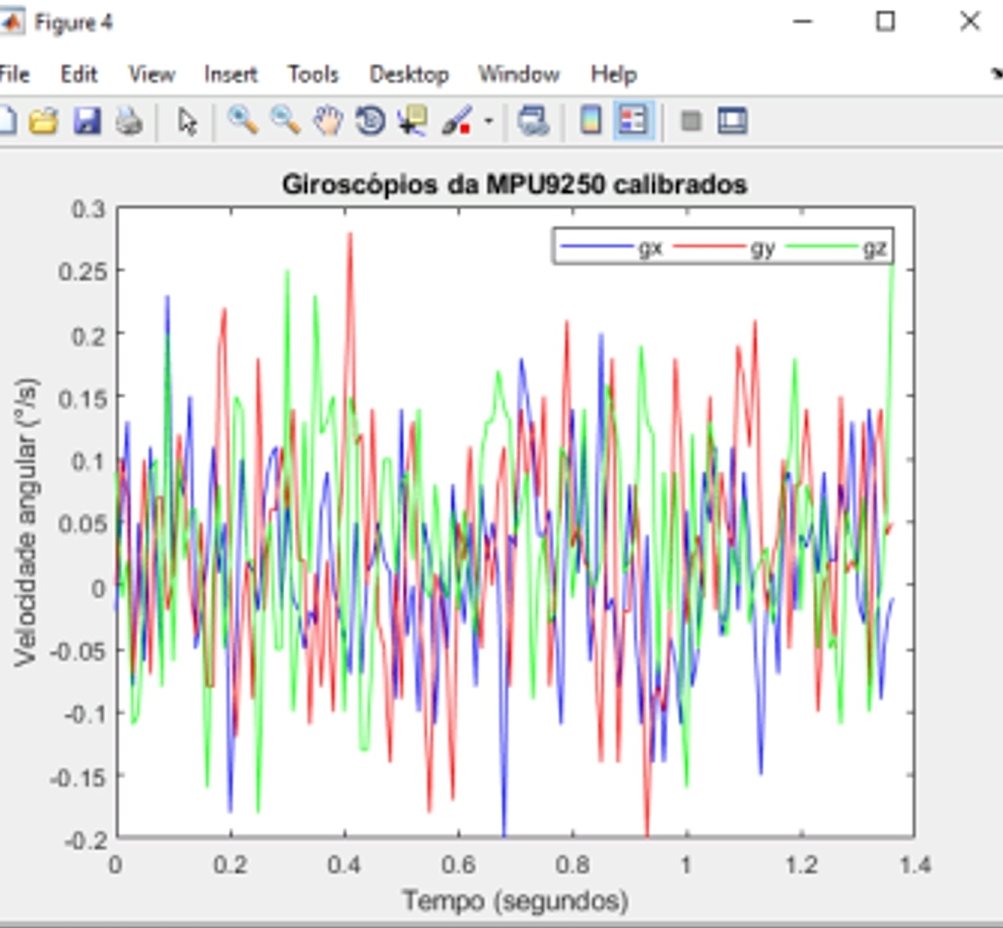
\includegraphics[width=7cm]{Figuras/giroscopio calibrado.jpeg}
\caption{Gráfica del giroscopio calibrado}
\label{fig:giroscopio calibrado}
\end{figure}
\section{Conexion VNC} \label{sec:VNC}
Para realizar las conexion VNC de la raspberry, se logra conectando el dispositivo desde donde se va a trabajar en este caso el PC a una red wifi a la que se debera conectar tambien la tarjeta, para ello deberemos disponer de 3 perifericos como lo son una pantalla, un teclado y un mouse que se utilizaran para en primer lugar para conectar la pi3 a la red de internet, luego procedemos a descargar el programa VNC en esta(raspberry) introduciremos posteriormente ifconfig para visualizar la IP y esta direccion la introduciremos en el programa VNC descargado con anterioridad en el PC utilizando el protocolo de comunicacion IP para realizar un control remoto de la raspberry pi3

%Para modificar las conclusiones se debe abrir y editar el archivo Conclusiones.tex
\section{Conclusiones} \label{sec:conclusiones}

Se logra la comunicación serial de la tarjeta de adquisición de datos con el PC.\\

Se observa que la tarjeta IMU presenta desvíos de fabrica y requiere ser calibrada.\\

Se logra mayor precisión en las lecturas con la tarjeta de adquisición mediante programación por medio de los offset.
 
 



%Para colocar una nueva sección se puede agregar en la ubicación que se desee después del titulo y antes de la bibliografía,
%se puede usar como modelo la siguiente configuración
%\input{Nueva_seccion}
%También se debe crear un nuevo archivo .tex con el mismo nombre anterior "Nueva_seccion" y dentro de este archivo se debe escribir lo %siguiente como primera línea
%\section{Nueva_seccion} \label{sec:Nueva_seccion}

%Como ultima configuración se incluye la bibliografía por medio de un archivo .bib que puede ser generado en mendeley y debe ser cargado %al proyecto
\bibliographystyle{IEEEtran}
\bibliography{bibfile}

\end{document}